%<<setup-child, include = FALSE>>=
%library(knitr)
%library(qrmix)
%library(mlr)
%library(quantreg)
%library(reshape2)
%set_parent("../style/preamble.Rnw")
%@


\documentclass[11pt,compress,t,notes=noshow, xcolor=table]{beamer}
\usepackage[]{graphicx}\usepackage[]{color}
% maxwidth is the original width if it is less than linewidth
% otherwise use linewidth (to make sure the graphics do not exceed the margin)
\makeatletter
\def\maxwidth{ %
  \ifdim\Gin@nat@width>\linewidth
    \linewidth
  \else
    \Gin@nat@width
  \fi
}
\makeatother

\definecolor{fgcolor}{rgb}{0.345, 0.345, 0.345}
\newcommand{\hlnum}[1]{\textcolor[rgb]{0.686,0.059,0.569}{#1}}%
\newcommand{\hlstr}[1]{\textcolor[rgb]{0.192,0.494,0.8}{#1}}%
\newcommand{\hlcom}[1]{\textcolor[rgb]{0.678,0.584,0.686}{\textit{#1}}}%
\newcommand{\hlopt}[1]{\textcolor[rgb]{0,0,0}{#1}}%
\newcommand{\hlstd}[1]{\textcolor[rgb]{0.345,0.345,0.345}{#1}}%
\newcommand{\hlkwa}[1]{\textcolor[rgb]{0.161,0.373,0.58}{\textbf{#1}}}%
\newcommand{\hlkwb}[1]{\textcolor[rgb]{0.69,0.353,0.396}{#1}}%
\newcommand{\hlkwc}[1]{\textcolor[rgb]{0.333,0.667,0.333}{#1}}%
\newcommand{\hlkwd}[1]{\textcolor[rgb]{0.737,0.353,0.396}{\textbf{#1}}}%
\let\hlipl\hlkwb

\usepackage{framed}
\makeatletter
\newenvironment{kframe}{%
 \def\at@end@of@kframe{}%
 \ifinner\ifhmode%
  \def\at@end@of@kframe{\end{minipage}}%
  \begin{minipage}{\columnwidth}%
 \fi\fi%
 \def\FrameCommand##1{\hskip\@totalleftmargin \hskip-\fboxsep
 \colorbox{shadecolor}{##1}\hskip-\fboxsep
     % There is no \\@totalrightmargin, so:
     \hskip-\linewidth \hskip-\@totalleftmargin \hskip\columnwidth}%
 \MakeFramed {\advance\hsize-\width
   \@totalleftmargin\z@ \linewidth\hsize
   \@setminipage}}%
 {\par\unskip\endMakeFramed%
 \at@end@of@kframe}
\makeatother

\definecolor{shadecolor}{rgb}{.97, .97, .97}
\definecolor{messagecolor}{rgb}{0, 0, 0}
\definecolor{warningcolor}{rgb}{1, 0, 1}
\definecolor{errorcolor}{rgb}{1, 0, 0}
\newenvironment{knitrout}{}{} % an empty environment to be redefined in TeX

\usepackage{alltt}
\newcommand{\SweaveOpts}[1]{}  % do not interfere with LaTeX
\newcommand{\SweaveInput}[1]{} % because they are not real TeX commands
\newcommand{\Sexpr}[1]{}       % will only be parsed by R
\newcommand{\xmark}{\ding{55}}%


\usepackage[english]{babel}
\usepackage[utf8]{inputenc}

\usepackage{dsfont}
\usepackage{verbatim}
\usepackage{amsmath}
\usepackage{amsfonts}
\usepackage{amssymb}
\usepackage{bm}
\usepackage{csquotes}
\usepackage{multirow}
\usepackage{longtable}
\usepackage{booktabs}
\usepackage{enumerate}
\usepackage[absolute,overlay]{textpos}
\usepackage{psfrag}
\usepackage{algorithm}
\usepackage{algpseudocode}
\usepackage{eqnarray}
\usepackage{arydshln}
\usepackage{tabularx}
\usepackage{placeins}
\usepackage{tikz}
\usepackage{setspace}
\usepackage{colortbl}
\usepackage{mathtools}
\usepackage{wrapfig}
\usepackage{bm}
\usepackage{amsmath}
\usepackage{pifont}
\usepackage[round]{natbib}
\usepackage{hyperref}

\usetikzlibrary{shapes,arrows,automata,positioning,calc,chains,trees, shadows}
\tikzset{
  %Define standard arrow tip
  >=stealth',
  %Define style for boxes
  punkt/.style={
    rectangle,
    rounded corners,
    draw=black, very thick,
    text width=6.5em,
    minimum height=2em,
    text centered},
  % Define arrow style
  pil/.style={
    ->,
    thick,
    shorten <=2pt,
    shorten >=2pt,}
}

\usepackage{subfig}

% Defines macros and environments
\usepackage{../../style/lmu-lecture}


\let\code=\texttt
\let\proglang=\textsf

\setkeys{Gin}{width=0.9\textwidth}

\setbeamertemplate{frametitle}{\expandafter\uppercase\expandafter\insertframetitle}

% basic latex stuff
\newcommand{\pkg}[1]{{\fontseries{b}\selectfont #1}} % fontstyle for R packages

% Often used in exercise Rnw files, still relevant?
\newcommand{\lz}{\vspace{0.5cm}} % vertical space
\newcommand{\dlz}{\vspace{1cm}}  % double vertical space

% Unused and about to be deleted
\newcommand{\oneliner}[1] % Oneliner for important statements
{\begin{block}{}\begin{center}\begin{Large}#1\end{Large}\end{center}\end{block}}


%--------------------%
%  New environments  %
%--------------------%

 % Frame with breaks and verbatim // this is used very often
\newenvironment{vbframe}
{
\begin{frame}[containsverbatim,allowframebreaks]
}
{
\end{frame}
}

% Frame with verbatim without breaks (to avoid numbering one slided frames)
% This is not used anywhere but I can see it being useful
\newenvironment{vframe}
{
\begin{frame}[containsverbatim]
}
{
\end{frame}
}

% Itemize block
\newenvironment{blocki}[1]
{
\begin{block}{#1}\begin{itemize}
}
{
\end{itemize}\end{block}
}

%--------------%
%  Citebutton  %
%--------------%
% Example usage (from slides-cart-discussion.tex)
% \citebutton{Breiman, 1984}{https://www.taylorfrancis.com/books/mono/10.1201/9781315139470/classification-regression-trees-leo-breiman}
\newcommand{\citebutton}[2]{%
\NoCaseChange{\resizebox{!}{9pt}{\protect\beamergotobutton{\href{#2}{#1}}}}%
}

% textcolor that works in mathmode
% https://tex.stackexchange.com/a/261480
% Used e.g. in forests/slides-forests-bagging.tex
% [...] \textcolor{blue}{\tfrac{1}{M}\sum^M_{m} [...]
\makeatletter
\renewcommand*{\@textcolor}[3]{%
  \protect\leavevmode
  \begingroup
    \color#1{#2}#3%
  \endgroup
}
\makeatother





% dependencies: amsmath, amssymb, dsfont
% math spaces
\ifdefined\N
\renewcommand{\N}{\mathds{N}} % N, naturals
\else \newcommand{\N}{\mathds{N}} \fi
\newcommand{\Z}{\mathds{Z}} % Z, integers
\newcommand{\Q}{\mathds{Q}} % Q, rationals
\newcommand{\R}{\mathds{R}} % R, reals
\ifdefined\C
\renewcommand{\C}{\mathds{C}} % C, complex
\else \newcommand{\C}{\mathds{C}} \fi
\newcommand{\continuous}{\mathcal{C}} % C, space of continuous functions
\newcommand{\M}{\mathcal{M}} % machine numbers
\newcommand{\epsm}{\epsilon_m} % maximum error

% counting / finite sets
\newcommand{\setzo}{\{0, 1\}} % set 0, 1
\newcommand{\setmp}{\{-1, +1\}} % set -1, 1
\newcommand{\unitint}{[0, 1]} % unit interval

% basic math stuff
\newcommand{\xt}{\tilde x} % x tilde
\DeclareMathOperator*{\argmax}{arg\,max} % argmax
\DeclareMathOperator*{\argmin}{arg\,min} % argmin
\newcommand{\argminlim}{\mathop{\mathrm{arg\,min}}\limits} % argmax with limits
\newcommand{\argmaxlim}{\mathop{\mathrm{arg\,max}}\limits} % argmin with limits
\newcommand{\sign}{\operatorname{sign}} % sign, signum
\newcommand{\I}{\mathbb{I}} % I, indicator
\newcommand{\order}{\mathcal{O}} % O, order
\newcommand{\bigO}{\mathcal{O}} % Big-O Landau
\newcommand{\littleo}{{o}} % Little-o Landau
\newcommand{\pd}[2]{\frac{\partial{#1}}{\partial #2}} % partial derivative
\newcommand{\floorlr}[1]{\left\lfloor #1 \right\rfloor} % floor
\newcommand{\ceillr}[1]{\left\lceil #1 \right\rceil} % ceiling
\newcommand{\indep}{\perp \!\!\! \perp} % independence symbol

% sums and products
\newcommand{\sumin}{\sum\limits_{i=1}^n} % summation from i=1 to n
\newcommand{\sumim}{\sum\limits_{i=1}^m} % summation from i=1 to m
\newcommand{\sumjn}{\sum\limits_{j=1}^n} % summation from j=1 to p
\newcommand{\sumjp}{\sum\limits_{j=1}^p} % summation from j=1 to p
\newcommand{\sumik}{\sum\limits_{i=1}^k} % summation from i=1 to k
\newcommand{\sumkg}{\sum\limits_{k=1}^g} % summation from k=1 to g
\newcommand{\sumjg}{\sum\limits_{j=1}^g} % summation from j=1 to g
\newcommand{\meanin}{\frac{1}{n} \sum\limits_{i=1}^n} % mean from i=1 to n
\newcommand{\meanim}{\frac{1}{m} \sum\limits_{i=1}^m} % mean from i=1 to n
\newcommand{\meankg}{\frac{1}{g} \sum\limits_{k=1}^g} % mean from k=1 to g
\newcommand{\prodin}{\prod\limits_{i=1}^n} % product from i=1 to n
\newcommand{\prodkg}{\prod\limits_{k=1}^g} % product from k=1 to g
\newcommand{\prodjp}{\prod\limits_{j=1}^p} % product from j=1 to p

% linear algebra
\newcommand{\one}{\bm{1}} % 1, unitvector
\newcommand{\zero}{\mathbf{0}} % 0-vector
\newcommand{\id}{\bm{I}} % I, identity
\newcommand{\diag}{\operatorname{diag}} % diag, diagonal
\newcommand{\trace}{\operatorname{tr}} % tr, trace
\newcommand{\spn}{\operatorname{span}} % span
\newcommand{\scp}[2]{\left\langle #1, #2 \right\rangle} % <.,.>, scalarproduct
\newcommand{\mat}[1]{\begin{pmatrix} #1 \end{pmatrix}} % short pmatrix command
\newcommand{\Amat}{\mathbf{A}} % matrix A
\newcommand{\Deltab}{\mathbf{\Delta}} % error term for vectors

% basic probability + stats
\renewcommand{\P}{\mathds{P}} % P, probability
\newcommand{\E}{\mathds{E}} % E, expectation
\newcommand{\var}{\mathsf{Var}} % Var, variance
\newcommand{\cov}{\mathsf{Cov}} % Cov, covariance
\newcommand{\corr}{\mathsf{Corr}} % Corr, correlation
\newcommand{\normal}{\mathcal{N}} % N of the normal distribution
\newcommand{\iid}{\overset{i.i.d}{\sim}} % dist with i.i.d superscript
\newcommand{\distas}[1]{\overset{#1}{\sim}} % ... is distributed as ...

% machine learning
\newcommand{\Xspace}{\mathcal{X}} % X, input space
\newcommand{\Yspace}{\mathcal{Y}} % Y, output space
\newcommand{\Zspace}{\mathcal{Z}} % Z, space of sampled datapoints
\newcommand{\nset}{\{1, \ldots, n\}} % set from 1 to n
\newcommand{\pset}{\{1, \ldots, p\}} % set from 1 to p
\newcommand{\gset}{\{1, \ldots, g\}} % set from 1 to g
\newcommand{\Pxy}{\mathbb{P}_{xy}} % P_xy
\newcommand{\Exy}{\mathbb{E}_{xy}} % E_xy: Expectation over random variables xy
\newcommand{\xv}{\mathbf{x}} % vector x (bold)
\newcommand{\xtil}{\tilde{\mathbf{x}}} % vector x-tilde (bold)
\newcommand{\yv}{\mathbf{y}} % vector y (bold)
\newcommand{\xy}{(\xv, y)} % observation (x, y)
\newcommand{\xvec}{\left(x_1, \ldots, x_p\right)^\top} % (x1, ..., xp)
\newcommand{\Xmat}{\mathbf{X}} % Design matrix
\newcommand{\allDatasets}{\mathds{D}} % The set of all datasets
\newcommand{\allDatasetsn}{\mathds{D}_n}  % The set of all datasets of size n
\newcommand{\D}{\mathcal{D}} % D, data
\newcommand{\Dn}{\D_n} % D_n, data of size n
\newcommand{\Dtrain}{\mathcal{D}_{\text{train}}} % D_train, training set
\newcommand{\Dtest}{\mathcal{D}_{\text{test}}} % D_test, test set
\newcommand{\xyi}[1][i]{\left(\xv^{(#1)}, y^{(#1)}\right)} % (x^i, y^i), i-th observation
\newcommand{\Dset}{\left( \xyi[1], \ldots, \xyi[n]\right)} % {(x1,y1)), ..., (xn,yn)}, data
\newcommand{\defAllDatasetsn}{(\Xspace \times \Yspace)^n} % Def. of the set of all datasets of size n
\newcommand{\defAllDatasets}{\bigcup_{n \in \N}(\Xspace \times \Yspace)^n} % Def. of the set of all datasets
\newcommand{\xdat}{\left\{ \xv^{(1)}, \ldots, \xv^{(n)}\right\}} % {x1, ..., xn}, input data
\newcommand{\ydat}{\left\{ \yv^{(1)}, \ldots, \yv^{(n)}\right\}} % {y1, ..., yn}, input data
\newcommand{\yvec}{\left(y^{(1)}, \hdots, y^{(n)}\right)^\top} % (y1, ..., yn), vector of outcomes
\newcommand{\greekxi}{\xi} % Greek letter xi
\renewcommand{\xi}[1][i]{\xv^{(#1)}} % x^i, i-th observed value of x
\newcommand{\yi}[1][i]{y^{(#1)}} % y^i, i-th observed value of y
\newcommand{\xivec}{\left(x^{(i)}_1, \ldots, x^{(i)}_p\right)^\top} % (x1^i, ..., xp^i), i-th observation vector
\newcommand{\xj}{\xv_j} % x_j, j-th feature
\newcommand{\xjvec}{\left(x^{(1)}_j, \ldots, x^{(n)}_j\right)^\top} % (x^1_j, ..., x^n_j), j-th feature vector
\newcommand{\phiv}{\mathbf{\phi}} % Basis transformation function phi
\newcommand{\phixi}{\mathbf{\phi}^{(i)}} % Basis transformation of xi: phi^i := phi(xi)

%%%%%% ml - models general
\newcommand{\lamv}{\bm{\lambda}} % lambda vector, hyperconfiguration vector
\newcommand{\Lam}{\bm{\Lambda}}	 % Lambda, space of all hpos
% Inducer / Inducing algorithm
\newcommand{\preimageInducer}{\left(\defAllDatasets\right)\times\Lam} % Set of all datasets times the hyperparameter space
\newcommand{\preimageInducerShort}{\allDatasets\times\Lam} % Set of all datasets times the hyperparameter space
% Inducer / Inducing algorithm
\newcommand{\ind}{\mathcal{I}} % Inducer, inducing algorithm, learning algorithm

% continuous prediction function f
\newcommand{\ftrue}{f_{\text{true}}}  % True underlying function (if a statistical model is assumed)
\newcommand{\ftruex}{\ftrue(\xv)} % True underlying function (if a statistical model is assumed)
\newcommand{\fx}{f(\xv)} % f(x), continuous prediction function
\newcommand{\fdomains}{f: \Xspace \rightarrow \R^g} % f with domain and co-domain
\newcommand{\Hspace}{\mathcal{H}} % hypothesis space where f is from
\newcommand{\fbayes}{f^{\ast}} % Bayes-optimal model
\newcommand{\fxbayes}{f^{\ast}(\xv)} % Bayes-optimal model
\newcommand{\fkx}[1][k]{f_{#1}(\xv)} % f_j(x), discriminant component function
\newcommand{\fh}{\hat{f}} % f hat, estimated prediction function
\newcommand{\fxh}{\fh(\xv)} % fhat(x)
\newcommand{\fxt}{f(\xv ~|~ \thetav)} % f(x | theta)
\newcommand{\fxi}{f\left(\xv^{(i)}\right)} % f(x^(i))
\newcommand{\fxih}{\hat{f}\left(\xv^{(i)}\right)} % f(x^(i))
\newcommand{\fxit}{f\left(\xv^{(i)} ~|~ \thetav\right)} % f(x^(i) | theta)
\newcommand{\fhD}{\fh_{\D}} % fhat_D, estimate of f based on D
\newcommand{\fhDtrain}{\fh_{\Dtrain}} % fhat_Dtrain, estimate of f based on D
\newcommand{\fhDnlam}{\fh_{\Dn, \lamv}} %model learned on Dn with hp lambda
\newcommand{\fhDlam}{\fh_{\D, \lamv}} %model learned on D with hp lambda
\newcommand{\fhDnlams}{\fh_{\Dn, \lamv^\ast}} %model learned on Dn with optimal hp lambda
\newcommand{\fhDlams}{\fh_{\D, \lamv^\ast}} %model learned on D with optimal hp lambda

% discrete prediction function h
\newcommand{\hx}{h(\xv)} % h(x), discrete prediction function
\newcommand{\hh}{\hat{h}} % h hat
\newcommand{\hxh}{\hat{h}(\xv)} % hhat(x)
\newcommand{\hxt}{h(\xv | \thetav)} % h(x | theta)
\newcommand{\hxi}{h\left(\xi\right)} % h(x^(i))
\newcommand{\hxit}{h\left(\xi ~|~ \thetav\right)} % h(x^(i) | theta)
\newcommand{\hbayes}{h^{\ast}} % Bayes-optimal classification model
\newcommand{\hxbayes}{h^{\ast}(\xv)} % Bayes-optimal classification model

% yhat
\newcommand{\yh}{\hat{y}} % yhat for prediction of target
\newcommand{\yih}{\hat{y}^{(i)}} % yhat^(i) for prediction of ith targiet
\newcommand{\resi}{\yi- \yih}

% theta
\newcommand{\thetah}{\hat{\theta}} % theta hat
\newcommand{\thetav}{\bm{\theta}} % theta vector
\newcommand{\thetavh}{\bm{\hat\theta}} % theta vector hat
\newcommand{\thetat}[1][t]{\thetav^{[#1]}} % theta^[t] in optimization
\newcommand{\thetatn}[1][t]{\thetav^{[#1 +1]}} % theta^[t+1] in optimization
\newcommand{\thetahDnlam}{\thetavh_{\Dn, \lamv}} %theta learned on Dn with hp lambda
\newcommand{\thetahDlam}{\thetavh_{\D, \lamv}} %theta learned on D with hp lambda
\newcommand{\mint}{\min_{\thetav \in \Theta}} % min problem theta
\newcommand{\argmint}{\argmin_{\thetav \in \Theta}} % argmin theta

% densities + probabilities
% pdf of x
\newcommand{\pdf}{p} % p
\newcommand{\pdfx}{p(\xv)} % p(x)
\newcommand{\pixt}{\pi(\xv~|~ \thetav)} % pi(x|theta), pdf of x given theta
\newcommand{\pixit}[1][i]{\pi\left(\xi[#1] ~|~ \thetav\right)} % pi(x^i|theta), pdf of x given theta
\newcommand{\pixii}[1][i]{\pi\left(\xi[#1]\right)} % pi(x^i), pdf of i-th x

% pdf of (x, y)
\newcommand{\pdfxy}{p(\xv,y)} % p(x, y)
\newcommand{\pdfxyt}{p(\xv, y ~|~ \thetav)} % p(x, y | theta)
\newcommand{\pdfxyit}{p\left(\xi, \yi ~|~ \thetav\right)} % p(x^(i), y^(i) | theta)

% pdf of x given y
\newcommand{\pdfxyk}[1][k]{p(\xv | y= #1)} % p(x | y = k)
\newcommand{\lpdfxyk}[1][k]{\log p(\xv | y= #1)} % log p(x | y = k)
\newcommand{\pdfxiyk}[1][k]{p\left(\xi | y= #1 \right)} % p(x^i | y = k)

% prior probabilities
\newcommand{\pik}[1][k]{\pi_{#1}} % pi_k, prior
\newcommand{\lpik}[1][k]{\log \pi_{#1}} % log pi_k, log of the prior
\newcommand{\pit}{\pi(\thetav)} % Prior probability of parameter theta

% posterior probabilities
\newcommand{\post}{\P(y = 1 ~|~ \xv)} % P(y = 1 | x), post. prob for y=1
\newcommand{\postk}[1][k]{\P(y = #1 ~|~ \xv)} % P(y = k | y), post. prob for y=k
\newcommand{\pidomains}{\pi: \Xspace \rightarrow \unitint} % pi with domain and co-domain
\newcommand{\pibayes}{\pi^{\ast}} % Bayes-optimal classification model
\newcommand{\pixbayes}{\pi^{\ast}(\xv)} % Bayes-optimal classification model
\newcommand{\pix}{\pi(\xv)} % pi(x), P(y = 1 | x)
\newcommand{\piv}{\bm{\pi}} % pi, bold, as vector
\newcommand{\pikx}[1][k]{\pi_{#1}(\xv)} % pi_k(x), P(y = k | x)
\newcommand{\pikxt}[1][k]{\pi_{#1}(\xv ~|~ \thetav)} % pi_k(x | theta), P(y = k | x, theta)
\newcommand{\pixh}{\hat \pi(\xv)} % pi(x) hat, P(y = 1 | x) hat
\newcommand{\pikxh}[1][k]{\hat \pi_{#1}(\xv)} % pi_k(x) hat, P(y = k | x) hat
\newcommand{\pixih}{\hat \pi(\xi)} % pi(x^(i)) with hat
\newcommand{\pikxih}[1][k]{\hat \pi_{#1}(\xi)} % pi_k(x^(i)) with hat
\newcommand{\pdfygxt}{p(y ~|~\xv, \thetav)} % p(y | x, theta)
\newcommand{\pdfyigxit}{p\left(\yi ~|~\xi, \thetav\right)} % p(y^i |x^i, theta)
\newcommand{\lpdfygxt}{\log \pdfygxt } % log p(y | x, theta)
\newcommand{\lpdfyigxit}{\log \pdfyigxit} % log p(y^i |x^i, theta)

% probababilistic
\newcommand{\bayesrulek}[1][k]{\frac{\P(\xv | y= #1) \P(y= #1)}{\P(\xv)}} % Bayes rule
\newcommand{\muk}{\bm{\mu_k}} % mean vector of class-k Gaussian (discr analysis)

% residual and margin
\newcommand{\eps}{\epsilon} % residual, stochastic
\newcommand{\epsv}{\bm{\epsilon}} % residual, stochastic, as vector
\newcommand{\epsi}{\epsilon^{(i)}} % epsilon^i, residual, stochastic
\newcommand{\epsh}{\hat{\epsilon}} % residual, estimated
\newcommand{\epsvh}{\hat{\epsv}} % residual, estimated, vector
\newcommand{\yf}{y \fx} % y f(x), margin
\newcommand{\yfi}{\yi \fxi} % y^i f(x^i), margin
\newcommand{\Sigmah}{\hat \Sigma} % estimated covariance matrix
\newcommand{\Sigmahj}{\hat \Sigma_j} % estimated covariance matrix for the j-th class

% ml - loss, risk, likelihood
\newcommand{\Lyf}{L\left(y, f\right)} % L(y, f), loss function
\newcommand{\Lypi}{L\left(y, \pi\right)} % L(y, pi), loss function
\newcommand{\Lxy}{L\left(y, \fx\right)} % L(y, f(x)), loss function
\newcommand{\Lxyi}{L\left(\yi, \fxi\right)} % loss of observation
\newcommand{\Lxyt}{L\left(y, \fxt\right)} % loss with f parameterized
\newcommand{\Lxyit}{L\left(\yi, \fxit\right)} % loss of observation with f parameterized
\newcommand{\Lxym}{L\left(\yi, f\left(\bm{\tilde{x}}^{(i)} ~|~ \thetav\right)\right)} % loss of observation with f parameterized
\newcommand{\Lpixy}{L\left(y, \pix\right)} % loss in classification
\newcommand{\Lpiv}{L\left(y, \piv\right)} % loss in classification
\newcommand{\Lpixyi}{L\left(\yi, \pixii\right)} % loss of observation in classification
\newcommand{\Lpixyt}{L\left(y, \pixt\right)} % loss with pi parameterized
\newcommand{\Lpixyit}{L\left(\yi, \pixit\right)} % loss of observation with pi parameterized
\newcommand{\Lhxy}{L\left(y, \hx\right)} % L(y, h(x)), loss function on discrete classes
\newcommand{\Lr}{L\left(r\right)} % L(r), loss defined on residual (reg) / margin (classif)
\newcommand{\lone}{|y - \fx|} % L1 loss
\newcommand{\ltwo}{\left(y - \fx\right)^2} % L2 loss
\newcommand{\lbernoullimp}{\ln(1 + \exp(-y \cdot \fx))} % Bernoulli loss for -1, +1 encoding
\newcommand{\lbernoullizo}{- y \cdot \fx + \log(1 + \exp(\fx))} % Bernoulli loss for 0, 1 encoding
\newcommand{\lcrossent}{- y \log \left(\pix\right) - (1 - y) \log \left(1 - \pix\right)} % cross-entropy loss
\newcommand{\lbrier}{\left(\pix - y \right)^2} % Brier score
\newcommand{\risk}{\mathcal{R}} % R, risk
\newcommand{\riskbayes}{\mathcal{R}^\ast}
\newcommand{\riskf}{\risk(f)} % R(f), risk
\newcommand{\riskdef}{\E_{y|\xv}\left(\Lxy \right)} % risk def (expected loss)
\newcommand{\riskt}{\mathcal{R}(\thetav)} % R(theta), risk
\newcommand{\riske}{\mathcal{R}_{\text{emp}}} % R_emp, empirical risk w/o factor 1 / n
\newcommand{\riskeb}{\bar{\mathcal{R}}_{\text{emp}}} % R_emp, empirical risk w/ factor 1 / n
\newcommand{\riskef}{\riske(f)} % R_emp(f)
\newcommand{\risket}{\mathcal{R}_{\text{emp}}(\thetav)} % R_emp(theta)
\newcommand{\riskr}{\mathcal{R}_{\text{reg}}} % R_reg, regularized risk
\newcommand{\riskrt}{\mathcal{R}_{\text{reg}}(\thetav)} % R_reg(theta)
\newcommand{\riskrf}{\riskr(f)} % R_reg(f)
\newcommand{\riskrth}{\hat{\mathcal{R}}_{\text{reg}}(\thetav)} % hat R_reg(theta)
\newcommand{\risketh}{\hat{\mathcal{R}}_{\text{emp}}(\thetav)} % hat R_emp(theta)
\newcommand{\LL}{\mathcal{L}} % L, likelihood
\newcommand{\LLt}{\mathcal{L}(\thetav)} % L(theta), likelihood
\newcommand{\LLtx}{\mathcal{L}(\thetav | \xv)} % L(theta|x), likelihood
\newcommand{\logl}{\ell} % l, log-likelihood
\newcommand{\loglt}{\logl(\thetav)} % l(theta), log-likelihood
\newcommand{\logltx}{\logl(\thetav | \xv)} % l(theta|x), log-likelihood
\newcommand{\errtrain}{\text{err}_{\text{train}}} % training error
\newcommand{\errtest}{\text{err}_{\text{test}}} % test error
\newcommand{\errexp}{\overline{\text{err}_{\text{test}}}} % avg training error

% lm
\newcommand{\thx}{\thetav^\top \xv} % linear model
\newcommand{\olsest}{(\Xmat^\top \Xmat)^{-1} \Xmat^\top \yv} % OLS estimator in LM


\usepackage{booktabs}

\newcommand{\titlefigure}{figure_man/vgg_example.png}
\newcommand{\learninggoals}{
  % \item Understand why you should care about properties of loss functions
  \item Know the concept of robustness 
  \item Learn about analytical and computational properties of loss functions 
  \item Understand that the loss function may influence convergence of the optimizer
}

\title{Introduction to Machine Learning}
% \author{Bernd Bi{}schl, Christoph Molnar, Daniel Schalk, Fabian Scheipl}
\institute{\href{https://compstat-lmu.github.io/lecture_i2ml/}{compstat-lmu.github.io/lecture\_i2ml}}
\date{}


\begin{document}

% ------------------------------------------------------------------------------

\lecturechapter{Properties of Loss Functions}
\lecture{Introduction to Machine Learning}

\begin{vbframe}{The role of Loss Functions}

Why should we care about how to choose the loss function $\Lxy$?

\begin{itemize}
% \item For regression, the loss usually only depends on residual $\Lxy = L\left(y - \fx\right) = L(\eps)$, this is a \emph{translation invariant} loss
\item \textbf{Statistical} properties: choice of loss implies statistical assumptions on the distribution of $y ~|~ \xv = \xv$ (see \emph{maximum likelihood estimation vs.
empirical risk minimization}). 
\item \textbf{Robustness} properties: some loss functions are more robust towards outliers than others. 
\item \textbf{Analytical} properties: the computational / optimization complexity of the problem. 
$$
\argmin_{\thetab \in \Theta} \risket
$$
is influenced by the choice of the loss function. 
\end{itemize}

\end{vbframe}

% ------------------------------------------------------------------------------

\begin{vbframe}{Basic Types of Regression Losses}

% https://davidrosenberg.github.io/mlcourse/Archive/2017/Lectures/3b.loss-functions.pdf

\begin{itemize}
  \small
  \item Regression losses usually only depend on the \textbf{ residuals}
  $r := y - \fx.$
  \item Classification losses are usually expressed in terms of the 
  \textbf{margin} $\nu := y \cdot \fx.$
  \item A loss is called \textbf{distance-based} if
  \begin{itemize}
    \small
    \item it can be written in terms of the residual
    $\Lxy = \psi (r) \text{ for some } \psi: \R \to \R, ~ \text{and}$
    \item $\psi(r) = 0 \Leftrightarrow r = 0$.
  \end{itemize}
  \item A loss is \textbf{translation-invariant} if $L(y + a, \fx + a) = \Lxy$.
  \item Losses are called \textbf{symmetric} if $\Lxy = L\left(\fx, y\right)$. 
\end{itemize}

\vfill

\begin{minipage}[b]{0.33\textwidth}
  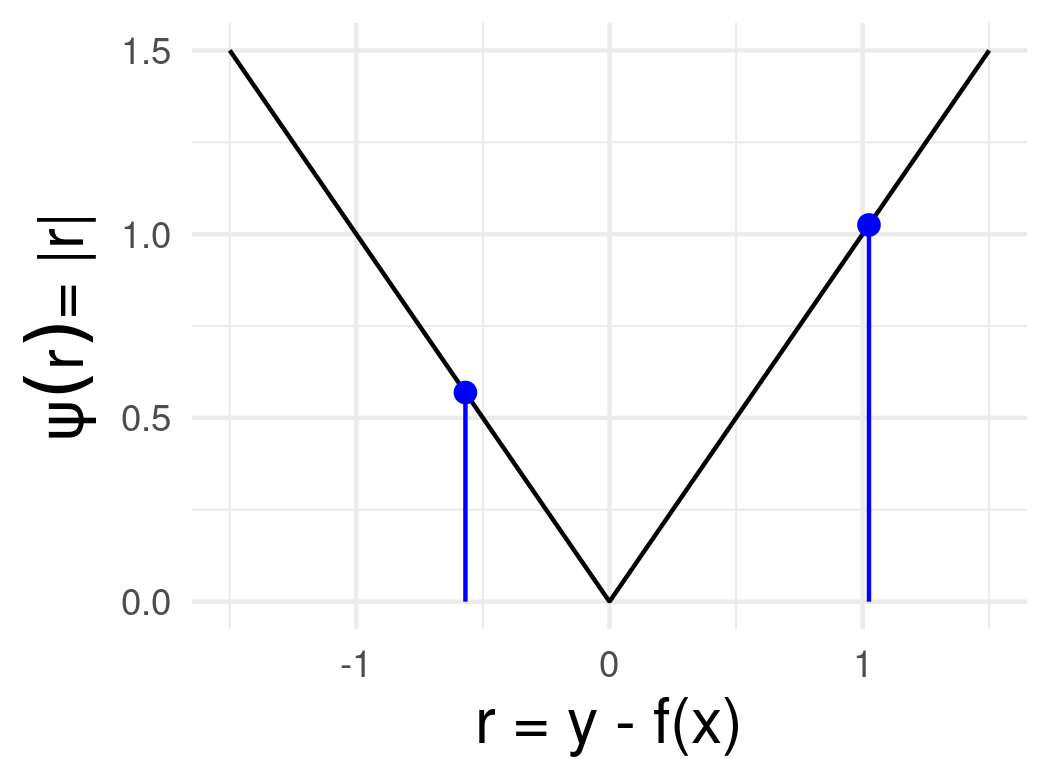
\includegraphics[width=\textwidth]{figure/loss_dist_based}
  \footnotesize \centering
  Distance-based: $L1$ loss
\end{minipage}%
\begin{minipage}[b]{0.33\textwidth}
  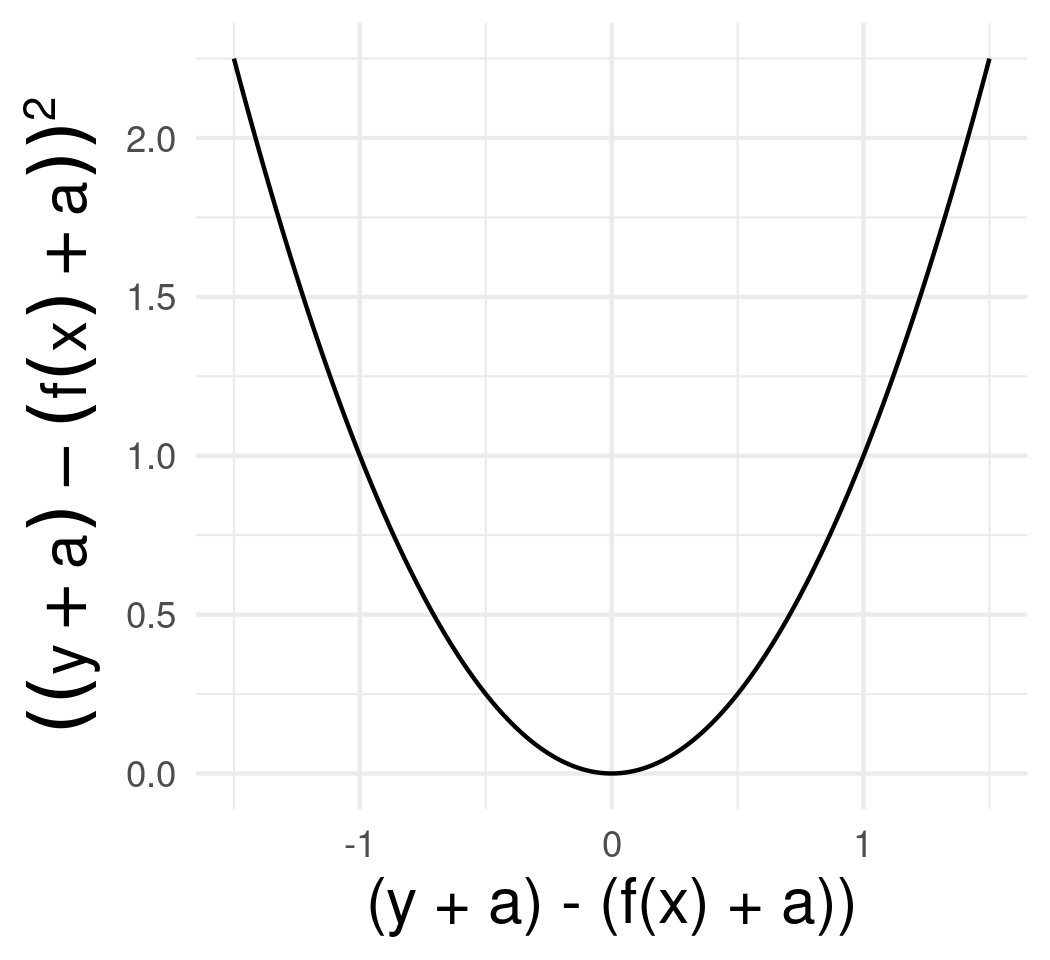
\includegraphics[width=\textwidth]{figure/loss_transl_inv.png}
  \footnotesize \centering
  Translation-invariant: $L2$ loss
\end{minipage}%
\begin{minipage}[b]{0.33\textwidth}
  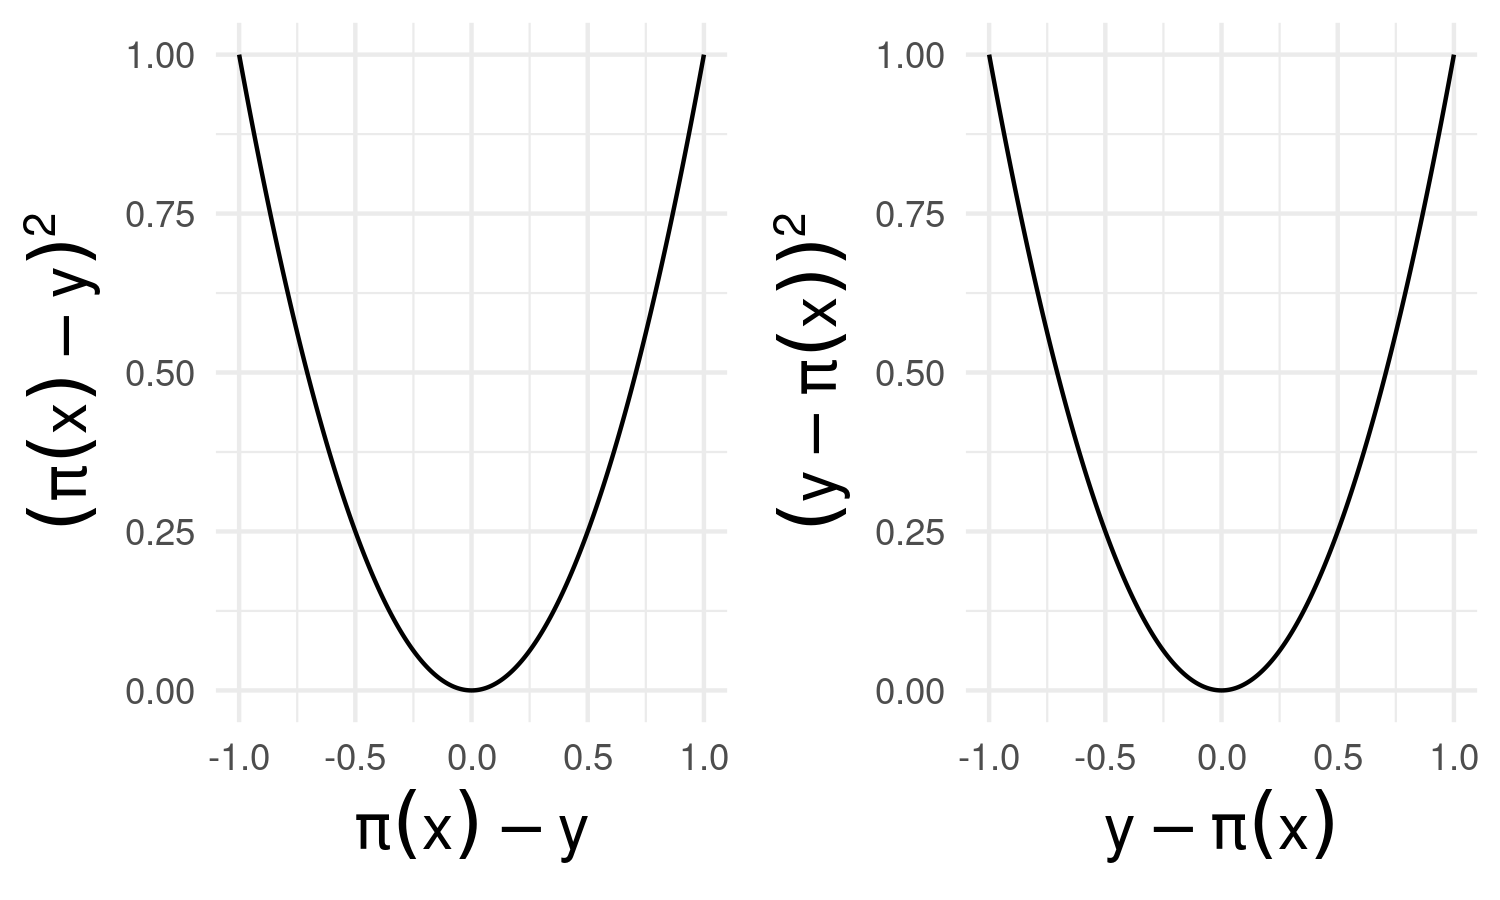
\includegraphics[width=\textwidth]{figure/loss_symmetric}
  \footnotesize \centering
  Symmetric: Brier score
\end{minipage}

\end{vbframe}

% ------------------------------------------------------------------------------

\begin{vbframe}{Robustness}

Outliers (in $y$) have large residuals $r = y - \fx$. For some losses large residuals have a much bigger impact on the risk much more than for other losses. 

\begin{table}[]
\begin{tabular}{lllll}
\toprule
$y$  & $\fxh$ & L1 & L2 & Huber ($\eps = 5$) \\ \midrule 
1 & 0 & 1 & 1 & 0.5 \\ 
5 & 0 & 5 & 25 & 12.5 \\ 
10 & 0 & 10 & 100 & 37.5 \\ 
50 & 0 & 50 & 2500  & 237.5 \\ \bottomrule
\end{tabular}
\end{table}

As a consequence, a model is less influenced by outliers than by inliers if the loss is robust. 

\textcolor{blue}{merge with subsequent slide}

\framebreak 

The L2 loss is an example for a loss function that is not very robust towards outliers. It penalizes large residuals more than the L1 or the Huber loss. The L1 and the Huber loss are thus regarded robust. 

\begin{center}
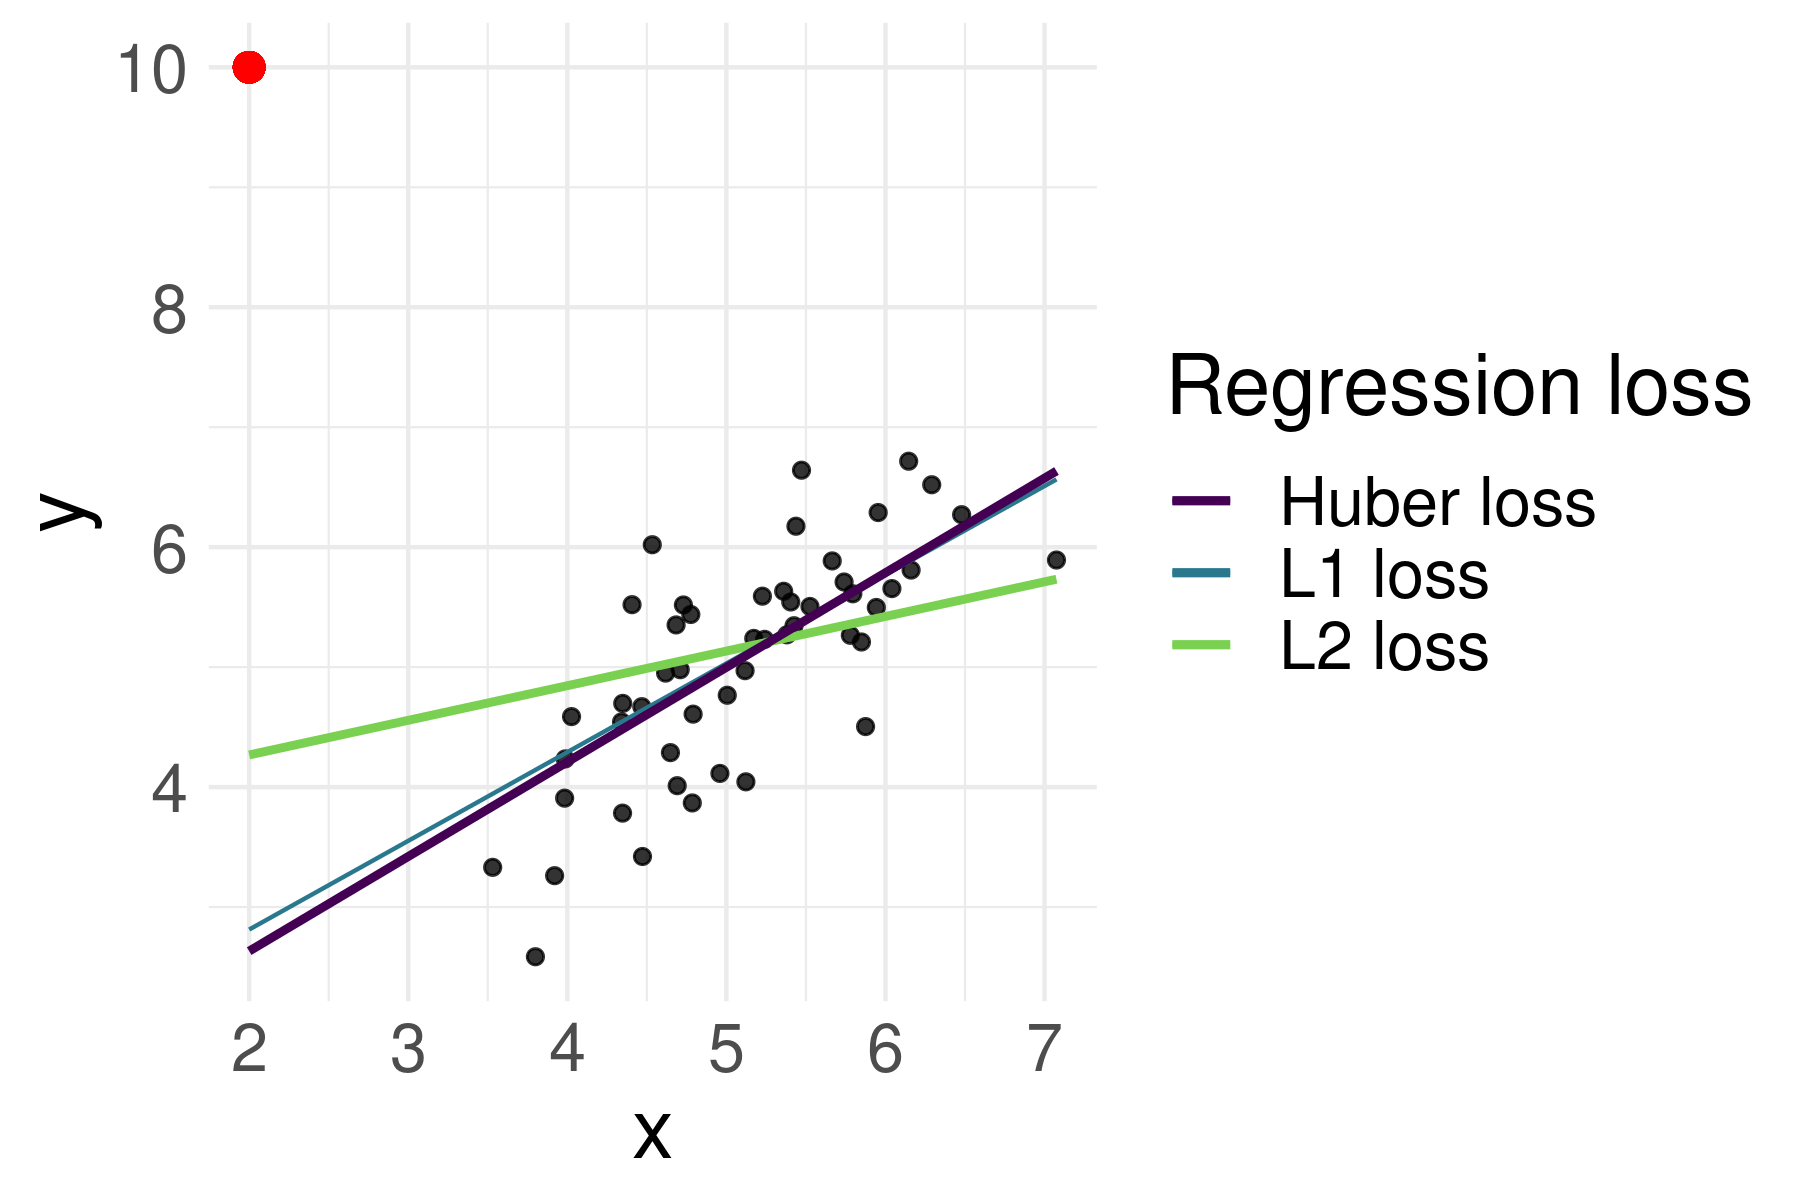
\includegraphics[width=0.8\textwidth]{figure/robustness.png}
\end{center}

\end{vbframe}

% ------------------------------------------------------------------------------

\begin{vbframe}{Analytical Properties: Smoothness}

\textcolor{blue}{LW: points 1-3 together w/ plot on subsequent slide; scnd slide w/ concrete examples (e.g., gd failing w/ lasso}

\begin{itemize}
    \item \textbf{Smoothness} of a function is a property that is measured by the number of continuous derivatives it has. 
    \item A function is said to be $\mathcal{C}^k$ if it is $k$ times continuously differentiable. A function is $\mathcal{C}^\infty$ if it is continuously differently for all orders $k$. 
    \item In contrast do derivative-free methods, derivative-based methods require a certain level of smoothness of the risk function $\risket$. 
    \item Example: Gradient descent requires differentiability of the $\risket$ (existence of $\nabla \risket$), Newton-Raphson requires $\risket$ to be twice differentiable (existence of Hessian $\nabla^2 \risket$). 

    \framebreak 

    \item If the loss function is not smooth, the risk minimization problem is in general not smooth either. 
    \item  Instead, derivative-free optimization need to be used (which might not be desirable)
\end{itemize}

\begin{center}
  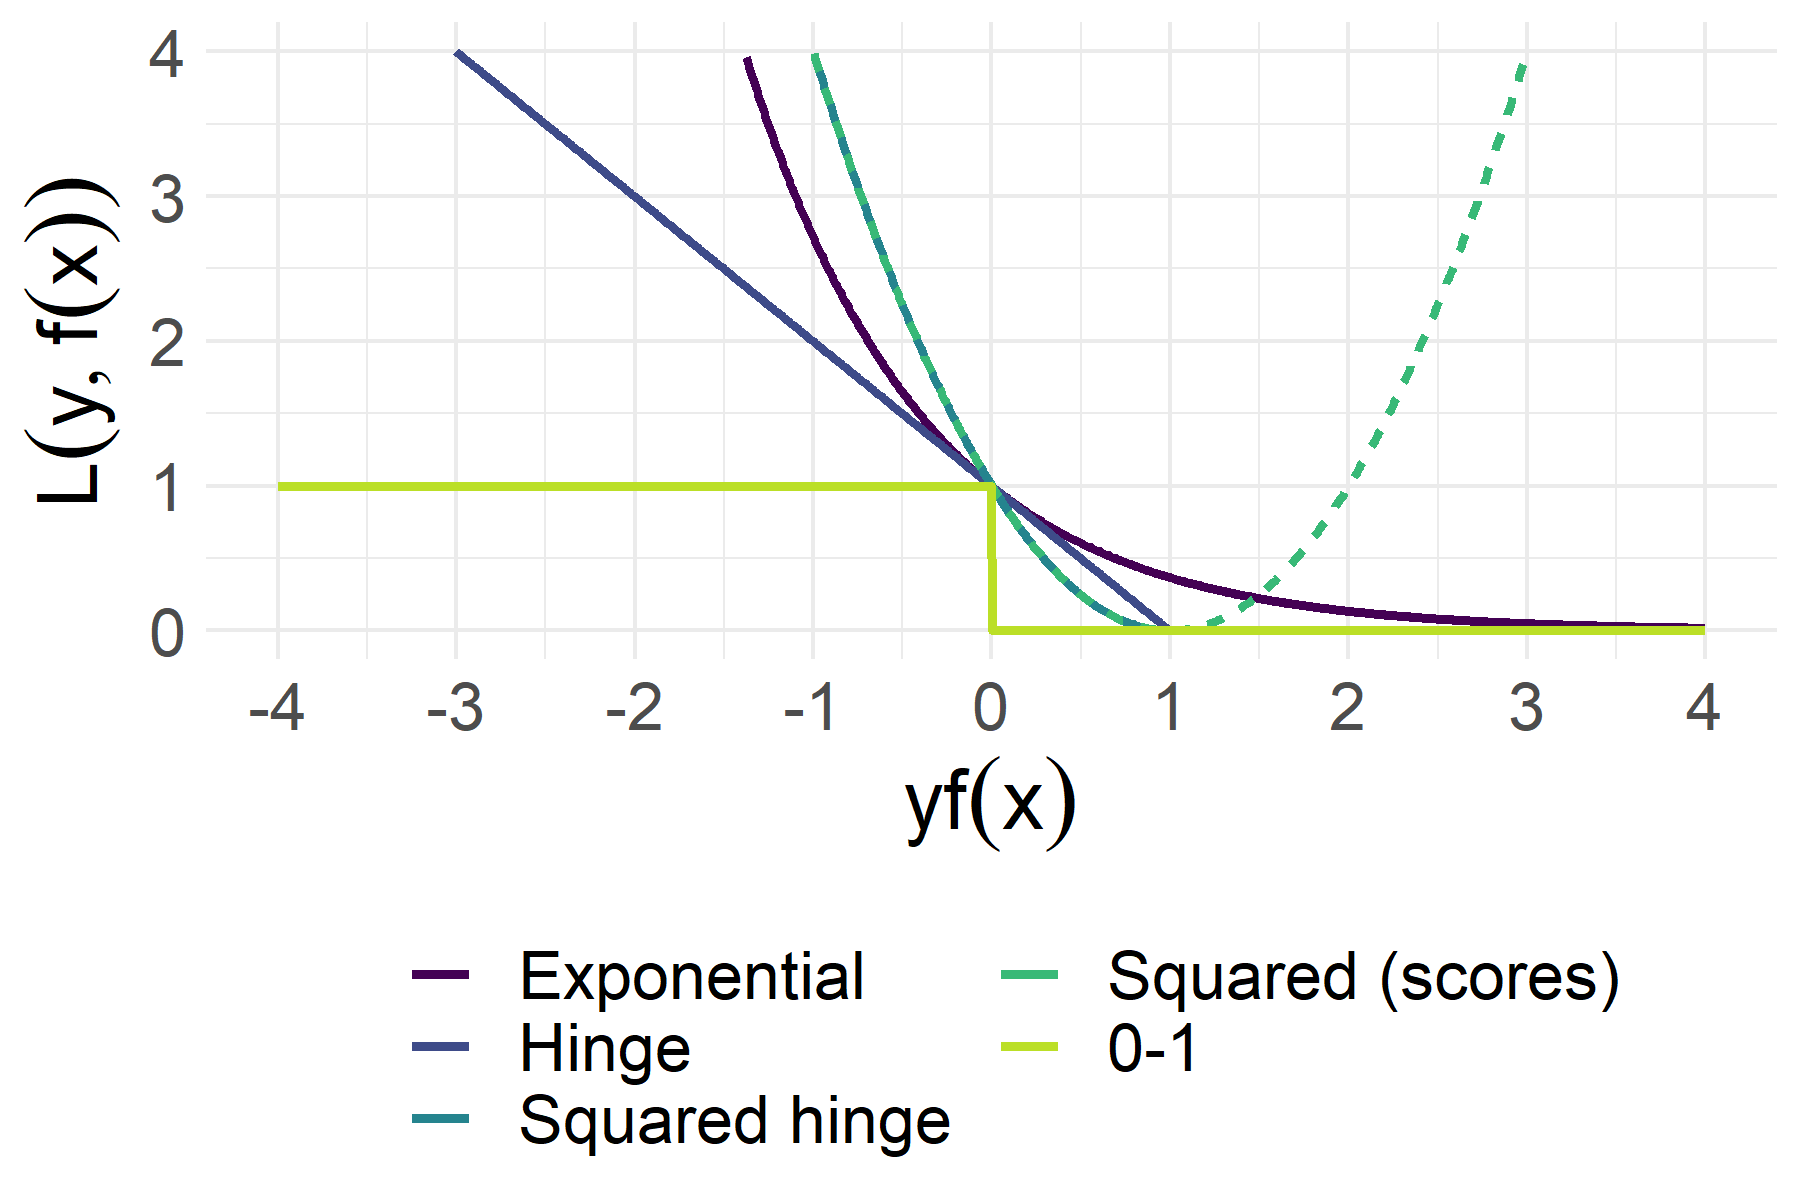
\includegraphics[width = 0.5\textwidth]{figure/plot_loss_overview_classif.png} \\
  \begin{footnotesize}
    Squared loss, exponential loss, and squared hinge loss are continuously differentiable. The hinge loss is continuous but not differentiable. The 0-1-loss is not even continuous.   
  \end{footnotesize}
\end{center}


%   \framebreak 
%   \item Convexity of loss functions
% \end{itemize}

\end{vbframe}

% ------------------------------------------------------------------------------

\begin{vbframe}{Analytical Properties: Convexity}

\textcolor{blue}{LW: add concrete examples of (non-)convex loss funs}

\begin{itemize}
  % \item A function $\risket$ is convex if 
  % $$
  %   \risk\left(t \thetab^{(1)} + (1 - t) \cdot \thetab^{(2)}\right) \le t \risk\left(\thetab^{(1)}\right) + (1 - t) \cdot \risk\left(\thetab^{(2)}\right) 
  % $$
  % for all $0 \le t \le 1$ and all $\thetab^{(1)}, \thetab^{(2)} \in \Theta$
  % (strictly convex if the above equation is fulfilled with equality). 
  \item In optimization, convex optimization problems are desirable because they have a number of conventient properties. In particular, it holds for convex problems: A local minimum of a convex function is also a global minimum. A strictly convex function has at most \textbf{one} global minimum (uniqueness). 
  \begin{center}
  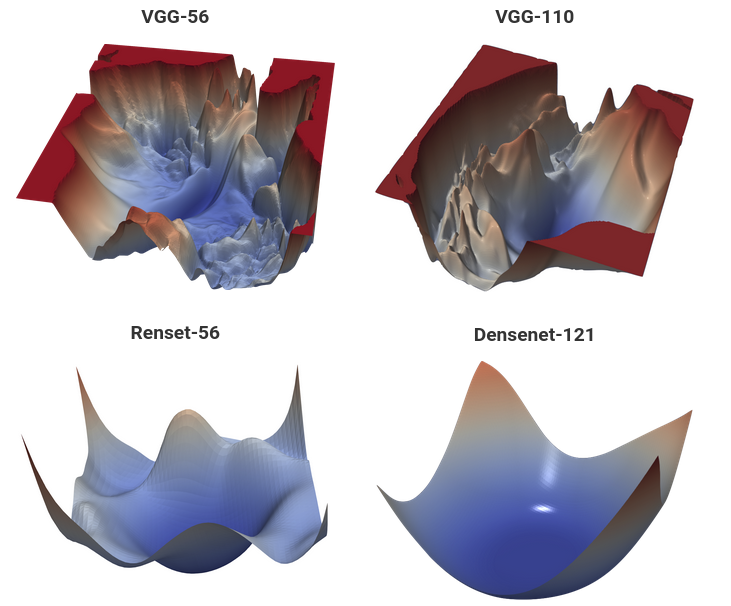
\includegraphics[width = 0.45\textwidth]{figure_man/convex-vs-nonconfex-landscape.png} \\
  \begin{footnotesize} Li et al., 2018, Visualizing the Loss Landscape of Neural Nets. The problem on the bottom right is convex, the others are not. \end{footnotesize}
  \end{center}
  \item In practical terms complexity means that we do not need to worry to get stuck in a local minimum during risk minimization. 
  \item Note that convexity of $\risket$ does not only depend on convexity of the loss function: Convexity of $\risket$ is also determined by the choice of the hypothesis space!
  \item For example, if $\Lxy$ is convex in its second argument, and $\fxt$ is linear in $\thetab$, then $\risket$ is convex. If $L$ is not convex, $\risket$ might have multiple local minima (bad!).
\end{itemize} 

\end{vbframe}

% ------------------------------------------------------------------------------

\begin{vbframe}{Analytical Properties: Convergence}

\textcolor{blue}{LW: not that much detail (belongs to logreg instead, is addressed in demo); story: if loss never reaches 0, w/ linearly separable data, it becomes desirable to have an infinitely steep logistic fun --> theta to infty}

\textcolor{red}{@BB: Do we want to cover this case here in such a detailed manner? }

The choice of the loss function may also imply convergence behavior of the optimization problem. 

\vspace*{0.2cm}

\textbf{Example: } Gradient descent will not converge if we minimize the Bernoulli loss for linearly separable data. 

\vspace*{0.2cm}

First, we take a look at logistic regression for an almost linearly separable dataset consisting of the observations $\xv^{(1)}, \dots, \xv^{(8)}$.
\vfill

\begin{figure}
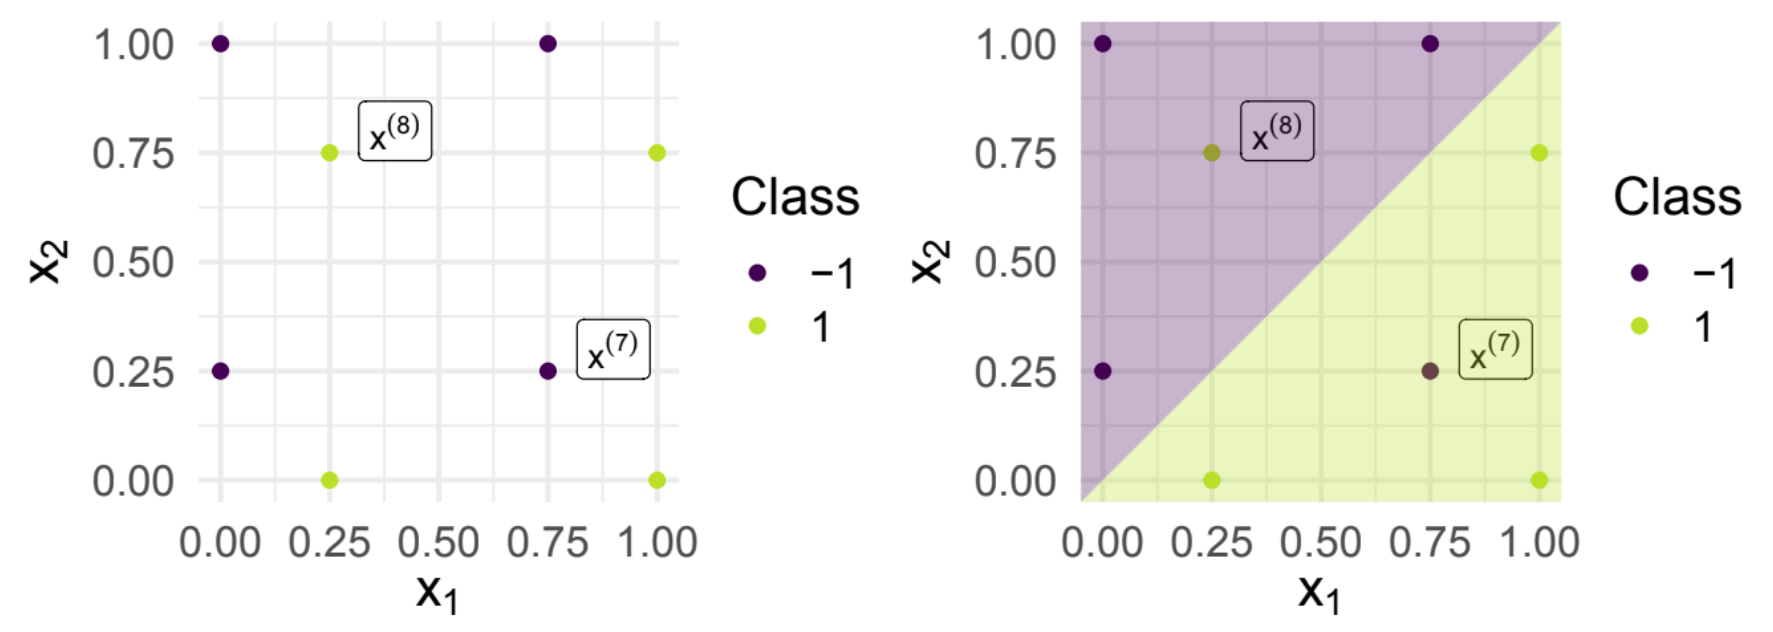
\includegraphics[width=0.9\textwidth]{figure_man/undet-problem01.png}\\
\end{figure}


Note: WLOG we estimate the
model without intercept, s.t. we can visualize the regression coefficient 
$\bm{\theta}$ in 2D. Also, the symmetry of the data does not influence the generality of our conclusions.

\vspace*{0.2cm}

Because of the symmetry of the data, the direction\footnote[frame]{$\bm{\theta}$ is perpendicular to the decision boundary and points to the "1"-space.} of $\bm{\theta}$ is $\tilde\thetab := (\frac{1}{\sqrt{2}}, -\frac{1}{\sqrt{2}})^\top$.

\medskip

To find $\overline{\theta} := ||\bm{\theta}||_2$, we consider the empirical risk $\riske$ along $\tilde\thetab$:
\begin{align*}
\riske &= \sum^8_{i=1} \log \left[1 + \exp \left(-y^{(i)}\thetab^\top \xv^{(i)}\right)\right] \\
&= \underbrace{\sum^6_{i=1} \log \left[1 + \exp \left(- \overline{\theta} \left|\tilde{\thetab}^\top \xv^{(i)}\right|\right)\right]}_{=: \; f_{\text{cor}}(\overline{\theta}) \;\text{(correctly classified)}} +
\underbrace{\sum^8_{i=7}\log \left[1 + \exp \left( \overline{\theta} \left| \tilde{\thetab}^\top \xv^{(i)}\right|\right)\right]}_{=:\; f_{\text{incor}}(\overline{\theta}) \;\text{(incorrectly classified)}}.
\end{align*}

\end{vbframe}

% ------------------------------------------------------------------------------

\begin{vbframe}{Analytical Properties: Convergence}

Clearly, $f_{\text{cor}}$ / $f_{\text{incor}}$ are monotonically decreasing/increasing with rising length of $\thetab$:

\begin{figure}
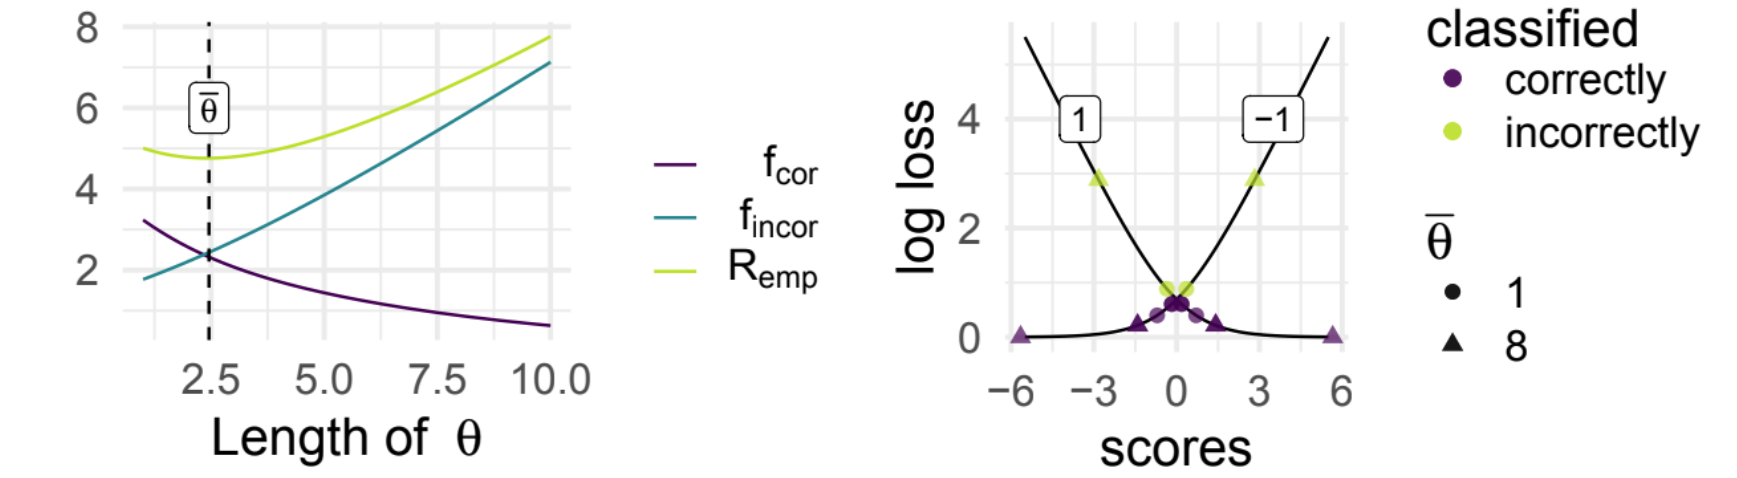
\includegraphics[width=0.8\textwidth]{figure_man/undet-problem02.png}\\
\end{figure}

\begin{itemize}
\item By removing obs. 7 and 8, we get a linearly separable dataset. \\
\item This also means that we lose our "counterweight", i.e., if a parameter vector $\thetab$ is able to classify the samples perfectly, the vector $2\thetab$ also classifies the samples perfectly, with decreased risk.
\item Therefore, an iterative optimizer such as gradient descent will continually increase $\thetab$ and never halt (in theory).
\item In such cases, regularization can guarantee convergence (see chapter on regularization). 
\end{itemize}

\end{vbframe}

% ------------------------------------------------------------------------------


% \begin{vbframe}{Visulizing Losses via Loss Plots}

% We call the plot that shows the point-wise error, i.e. the loss $\Lxy$ vs. the \textbf{residuals} $\eps := y - \fx$ (for regression), \textbf{loss plot}. The pseudo-residual corresponds to the slope of the tangent in $\left(y - \fx, \Lxy \right)$. 

% \vspace*{0.5cm}


% \begin{figure}
% 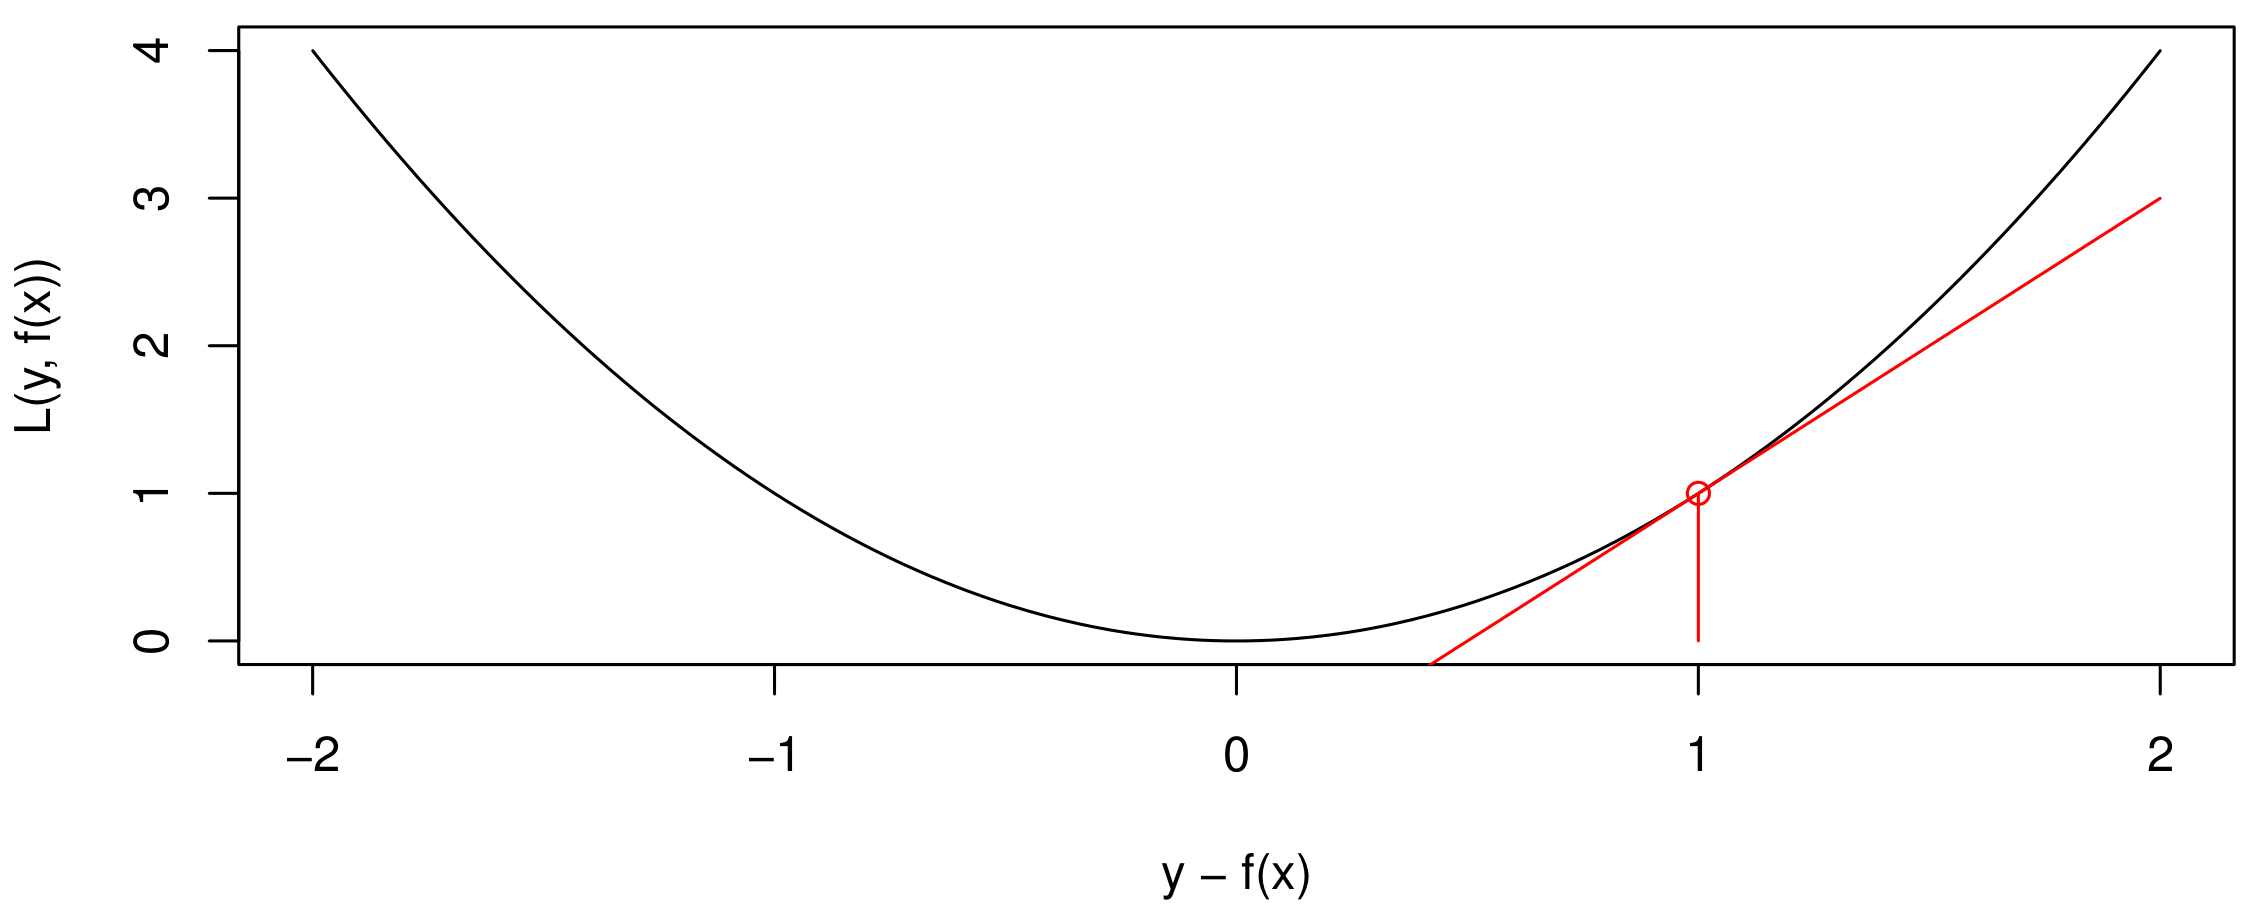
\includegraphics[width = 1\linewidth]{figure_man/loss.png}
% \end{figure}

% %<<echo=FALSE, warning=FALSE, message=FALSE, fig.height = 4>>=
% %   xx = seq(-2, 2, by = 0.01); 
% %   yy = xx^2
% %   plot(xx, yy, type = "l", xlab = "y - f(x)", ylab = "L(y, f(x))")
% %   points(1, 1, col = "red")
% %   lines(x = c(1, 1), y = c(0, 1), col = "red")
% %   points(xx, 2 * xx - 1, type = "l", col = "red")
% %  @

% % We will define a similar plot for classification later on in this chapter.

% \end{vbframe}










% \section{Comparison of Loss Functions}
% 
% 
% \begin{vbframe}{Comparison of Loss Functions}
% 
% 
% \begin{center}
% \includegraphics[width = 10cm]{figure_man/2_7_loss_comparison_plot1.png} \\
% \end{center}
% 
% 
% \framebreak
% 
% 
% This plot shows the optimal constant model $\fx = \thetab$ (also \enquote{featureless predictor}) for the losses that have been discussed.
% 
% \begin{center}
% \includegraphics[width = 10cm, height = 6.5cm]{figure_man/2_8_loss_comparison_constant_model_plot1.png} \\
% \end{center}
% 
% \end{vbframe}




\endlecture

\end{document}